Uraikan semua dasar teori pendukung tugas akhir ini dengan terstruktur dan sistematis. Terstruktur dan sistematis artinya semua teori yang diperlukan dapat disajikan dengan urutan yang baik sehingga tidak terjadi perulangan di belakang. Misalnya teori dan semua variabel setelah dideklarasikan, maka akan dipakai seterusnya tanpa mengulangi definisi teori dan variabel tersebut kecuali jika secara spesifik diperlukan. 

Walaupun berupa dasar teori, tim \textit{capstone} \uline{harus menuliskannya sendiri} dan \textbf{\uline{dilarang keras} \uline{untuk melakukan \textit{copy and paste}}} serta \uline{wajib bebas dari plagiarisme}. Menyunting diperbolehkan selama memenuhi kriteria akademis dengan memberikan referensi yang tepat. Mahasiswa diharapkan untuk bisa belajar tentang etika akademik yang berkaitan dengan cara menyunting untuk menghindari praktek plagiarisme kepada dosen pembimbing \textit{capstone} masing-masing.

Sebagai contoh, berikut ini adalah dasar teori yang menjelaskan mengenai interpretasi geometris dari konsep \textit{eigenvalue} dan \textit{eigenvector}.

\section{Intepretasi Geometris dari \textit{Eigenvalues} dan \textit{Eigenvectors}}
\label{sec:Interpretasi_Geometris_Eigenvalue_Eigenvector}

    Dalam ilmu Aljabar Linear, ketika sebuah matriks $A$ dikalikan dengan sebuah vektor $v$, makna dari proses perkalian tersebut adalah matriks $A$ tersebut mentransformasikan vektor $v$ menjadi sebuah vektor baru $w = T(v) = Av$. Ide dari transformasi $T(v)$ tersebut sama dengan ide dari fungsi $y = f(x)$, yang mana akan menghasilkan sebuah nilai baru $y$ ketika kita memasukkan sebuah nilai tertentu $x$ ke dalam fungsi tersebut. 
    
    \begin{figure}[h!]
        \centering
        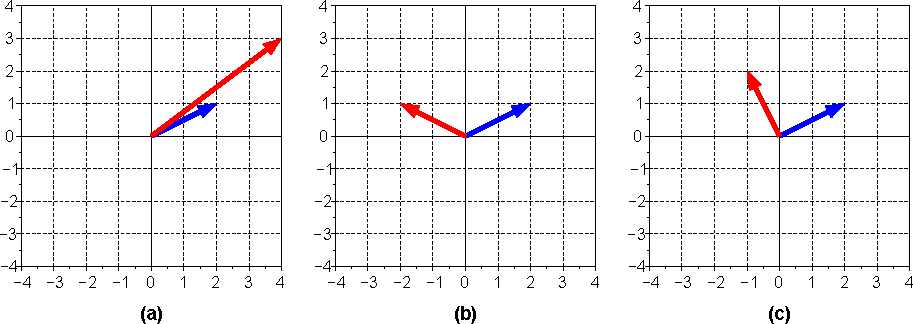
\includegraphics[scale=1.0]{Ch02_Vector_Transformation.pdf}
        \caption{Efek dari 3 Matriks Transformasi yang Berbeda terhadap Vektor $v$ (Biru)}
        \label{fig:Ch02_Vector_Transformation}
    \end{figure}
        
    Macam dari matriks transformasi $A$ tersebut sangatlah banyak, antara lain :
    \begin{equation}
    	\label{eqn:Ch02_Transformation_Matrix}
    	\begin{split}
    		A_1 =
    		\begin{bmatrix}
    			2 & 0 \\ 0 & 3
    		\end{bmatrix}
    		\quad \text{;} \quad
    		A_2 =
    		\begin{bmatrix}
    			-1 & 0 \\ 0 & 1
    		\end{bmatrix}
    		\quad \text{;} \quad
    		A_3 =
    		\begin{bmatrix}
    			0 & -1 \\ 1 & 0
    		\end{bmatrix}
    	\end{split}
    \end{equation}
    Representasi grafis dari masing-masing matriks transformasi tersebut dapat dilihat pada Gambar \ref{fig:Ch02_Vector_Transformation}. Seperti yang ditunjukkan pada Gambar \ref{fig:Ch02_Vector_Transformation}(a), matriks transformasi $A_1$ merupakan sebuah matriks \textit{scaling}, yang mengubah panjang komponen sumbu $x$ dari vektor $v$ menjadi 2 kalinya, dan panjang komponen sumbu $y$ dari vektor $v$ menjadi 3 kalinya. Sedangkan untuk matriks transformasi $A_2$, matriks ini digunakan untuk mencerminkan vektor $v$ terhadap sumbu $y$ seperti yang ditunjukkan oleh Gambar \ref{fig:Ch02_Vector_Transformation}(b). Terakhir, untuk matriks transformasi $A_3$ merupakan matriks rotasi, yang merotasi vektor $v$ sejauh $90^o$ dengan arah berlawanan dengan arah jarum jam seperti yang ditunjukkan oleh Gambar \ref{fig:Ch02_Vector_Transformation}(c).
    